\chapter{Analyse}
\label{chap:anal}
Notre implémentation comprend notamment une représentation binaire, aussi appelé Bitboard, les algorithmes de recherches Minimax et Alpha-Beta, et un classifieur pour prédire le résultat d'une partie en cours. Nous détaillons également les structures de données utilisées, et les algorithmes de décalage pour les coups valides. Nous avons réalisé ce projet en Python, pour des raisons de simplicité et de rapidité de développement, notamment à propos de la visualisation, et du développement du modèle de deep learning via PyTorch\footnote{PyTorch est une bibliothèque de tenseurs optimisée pour l'apprentissage profond. Voir \href{https://pytorch.org/docs/stable/index.html}{Documentation PyTorch}.}.

% Dans la littérature, un `coup` est souvent défini comme l'action des deux joueurs pendant un tour, et un `demi-coup` comme l'action d'un seul joueur. Cependant, dans le cadre de ce rapport, nous utiliserons plutôt le terme `coup` pour désigner le fait de poser un pion.


\section{Modélisation et structures de données}
\label{sec:mod}

\subsection{Structure du projet}
\label{subsec:struct}
\dirtree{%
.1 \textbf{Othello-Reversi/}.
.2 config.yaml : fichier de configuration des paramètres globaux du projet.
.2 \texttt{main} : point d'entrée du programme, permet de réaliser des tests, lancer des parties, faire jouer des algorithmes, etc.
.2 \texttt{game.py} : contient la logique de la boucle de jeu, permet de lancer une partie selon les paramètres donnés.
.2 \texttt{node.py} : contient la classe $\texttt{Node}$, encapsulant un état du jeu, et les informations nécessaires pour l'exploration de l'arbre de recherche, ou pour rejouer une partie.
.2 \texttt{strategies.py} : contient les algorithmes de recherche, et retourne le plateau après jouer un coup selon la stratégie choisie.
.2 \texttt{next.py} : contient les fonctions de calcul des coups valides, et celles pour jouer un coup.
.2 \texttt{heuristics.py} : contient les fonctions d'évaluation basées sur des heuristiques.
.2 \textbf{utils/}.
.3 \textit{Ensemble de fonctions utilitaires} telles que des tables d'heuristiques, la visualisation, les opérations logiques, etc.
.2 \texttt{model\_pipeline.ipynb} : notebook Jupyter pour data preprocessing, model training, et evaluation.
.2 \texttt{understanding\_bitboards.ipynb} : notebook Jupyter pour comprendre les bitboards, de nombreux exemples illustrent les opérations logiques.
}\leavevmode\\

Une partie peut être lancée depuis le programme \texttt{main.py}, ce dernier prendra les paramètres définies dans le fichier \texttt{config.yaml}. Par exemple, pour lancer une partie avec \textit{Interface} entre un joueur \textit{Humain} et un joueur \textit{Negamax-AlphaBeta}, en utilisant une stratégie \textit{Positionnelle} pour l'évaluation avec une profondeur d'exploration maximale de 4 coups, nous obtenons le fichier de configuration suivant: 
\begin{figure}[H]
    \centering
    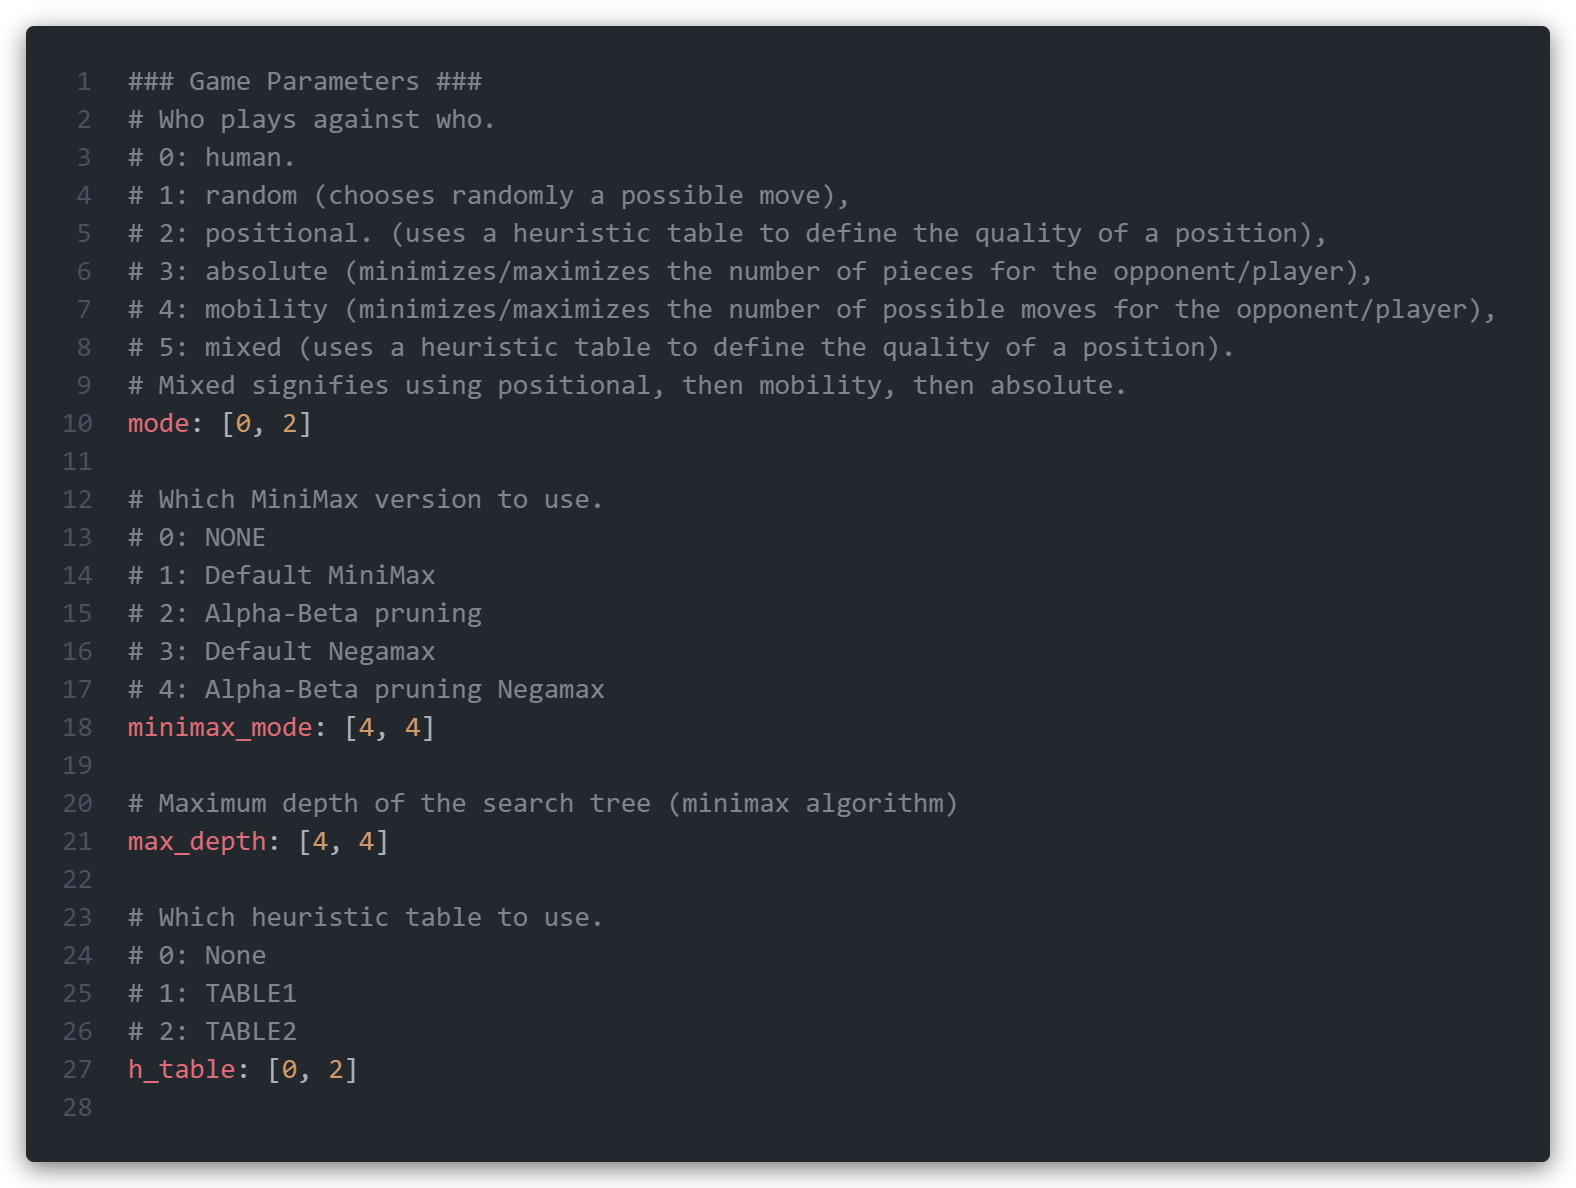
\includegraphics[width=\textwidth]{ressources/configYaml.png}
    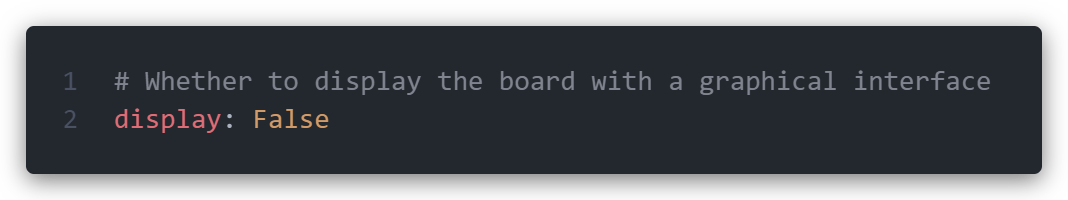
\includegraphics[width=\textwidth]{ressources/configYaml-display.png}
    \caption{Exemple d'une configuration (non complète).}
    \label{fig:configYaml}
\end{figure}

Plus de paramètres sont disponibles, accompagnés de leurs valeurs par défaut, ainsi que des descriptions et commentaires.


\subsection{Bitboards}
\label{subsec:bit}
Une représentation classique d'un plateau de jeu d'Othello est une matrice de 8x8, où chaque case peut contenir trois valeurs : par exemple (-1, 0, 1) pour les pions noirs, vides et blancs respectivement. Celle-ci est intuitive, et est la première approche que nous avions envisagée. Cependant, nous avons finalement opté pour une meilleure alternative, plus efficace en termes de temps et d'espace : les bitboards.

En effet, au lieu de contenir 64 entiers de $32 bits$ chacun (soit $2048 bits$), nous pouvons encoder l'ensemble du plateau de jeu dans 2 entiers de $64 bits$ chacun (soit $128bits$) : ce qui est 16 fois moins lourd ! 

De plus, les opérations logiques sur les bitboards sont très rapides, un avantage supplémentaire pour les algorithmes de recherche.

\subsubsection{Comment encoder un pion, un coup, ou un plateau de jeu ?}
\label{subsubsec:enc}
Nous pouvons en fait tous les encoder de la même manière, à travers un entier sur $64bits$. Chaque bit représente une case du plateau, sa valeur égale à 1 si elle est occupée par un pion, ou si le coup est valide. Le \ac{MSB} correspond à la case $h8$, et le \ac{LSB} à la case $a1$. Les positions sont usuellement notés de $a1$ à $h8$, où $a$ est la colonne la plus à gauche, et $1$ la ligne la plus haute. \cite{brian_rose_2005} 

Par exemple, la configuration initiale du plateau de jeu est la suivante :
\begin{itemize}
    \item Les pions noirs sont en $d5$ et $e4$.
    \item Les pions blancs sont en $d4$ et $e5$.
\end{itemize}

\begin{figure}[H]
    \centering
    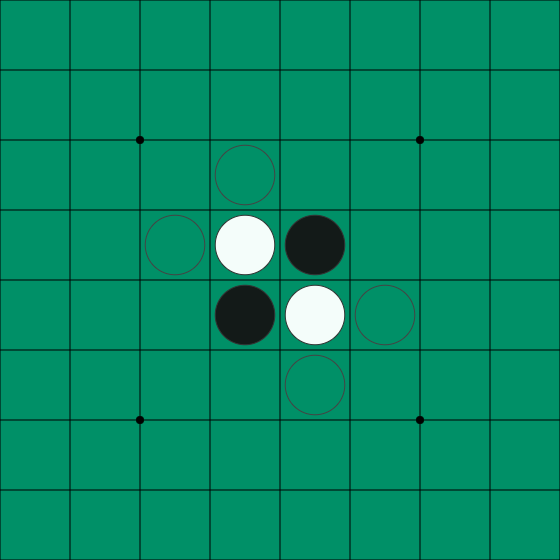
\includegraphics[width=0.5\textwidth]{ressources/plateau_init.png}
    \caption{Configuration initiale du plateau de jeu. Source : \href{https://www.eothello.com/}{eOthello}.}
    \label{fig:init_board}
\end{figure}

Cette dernière s'encode comme suit, avec dans l'ordre, le plateau noir, puis blanc :

\begin{center}
$0b00000000\_00000000\_00000000\_00001000\_00010000\_00000000\_00000000\_00000000$ \\
$0b00000000\_00000000\_00000000\_00010000\_00001000\_00000000\_00000000\_00000000$ \\
\end{center}
Ces deux entiers peuvent être réécris en hexadécimal pour une meilleure lisibilité :
\begin{align*}
    &0x00\_00\_00\_08\_10\_00\_00\_00 \quad (noir)\\
    &0x00\_00\_00\_10\_08\_00\_00\_00 \quad (blanc)\\
\end{align*}

De fait, il est possible de récupérer la valeur de la case $c_{i,j}$ d'un bitboard $b$ en utilisant la formule suivante : 
\begin{align*}
    (b\quad \gg\quad (8\times i+j))\quad \&\quad 1, \quad \forall i,j \in \{0,\dots,7\}
\end{align*}
Avec $i$ la ligne, $j$ la colonne, $\gg$ l'opérateur de décalage à droite, et $\&$ l'opérateur logique '\texttt{et}'.

Similairement, nous pouvons définir la case $c_{i,j}$ d'un bitboard $b$ en utilisant la formule suivante :
\begin{align*}
    b\quad |\quad (1\quad \ll\quad (8\times i+j)), \quad \forall i,j \in \{0,\dots,7\}
\end{align*}
Avec $\ll$ l'opérateur de décalage à gauche, et $|$ l'opérateur logique '\texttt{ou}'.

Nous obtenons toutes les pièces posées et toutes les cases vides avec les opérations logiques suivantes :
\begin{align*}
    \text{pieces} &= \text{noir} \quad | \quad \text{blanc} \\
    \text{vides} &= \quad\sim\text{pieces}
\end{align*}
Avec $\sim$ l'opérateur logique 'non'. Les programmes équivalents en python sont donnés dans l'appendice \ref{app:logical_ops}. De manière générale, n'importe quel pion peut être ajouté au plateau avec l'opérateur logique '\texttt{ou}'. Aussi, \texttt{8} peut être remplacé par n'importe quel entier représentant la taille du plateau, ici \texttt{8x8}.

\subsection{Structure Node}
\label{subsec:node}
Dans le contexte de ce projet, nous aimerions pouvoir rejouer des parties, déterminer les états déjà traités, et reprendre les anaylyses formulés lors de tours précédants. Pour cela, nous avons défini une structure de données nommée \texttt{Node}, qui encapsule un état du jeu, et les informations nécessaires pour l'exploration de l'arbre de recherche. Nous l'avons défini dans le fichier \texttt{node.py} via une classe Python. \vskip 0.5cm

\noindent\textbf{Attributs:}
\begin{itemize}
    \item \textbf{parent} : Référence au nœud parent dans l'arbre de jeu.
    \item \textbf{pièces\_joueur} : Représente les pièces du joueur actuel (bitboard).
    \item \textbf{pièces\_ennemi} : Représente les pièces de l'ennemi. (bitboard)
    \item \textbf{tour} : Indique à qui est le tour de jouer (-1 pour noir, 1 pour blanc).
    \item \textbf{taille} : La taille du plateau de jeu.
    \item \textbf{enfants} : Liste des nœuds enfants générés par expansion.
    \item \textbf{coups} : Liste des coups possibles à partir de ce nœud.
    \item \textbf{directions} : Dictionnaire associant à chaque coup les directions des pièces à capturer.
    \item \textbf{coups\_vers\_enfant} : Dictionnaire reliant les coups aux nœuds enfants correspondants.
    \item \textbf{valeur} : Valeur évaluative du nœud pour les algorithmes de recherche.
    \item \textbf{visité} : Booléen indiquant si le nœud a été visité lors de la recherche.
\end{itemize}
\leavevmode\\
\textbf{Méthodes:}
\begin{itemize}
    \item \textbf{développer()} : Génère tous les coups possibles et prépare les structures pour l'expansion.
    \item \textbf{définir\_enfant(coup)} : Crée un nœud enfant à partir d'un coup spécifié et l'ajoute à la liste des enfants. Si le noeud enfant existe déjà, il est simplement retourné.
    \item \textbf{ajouter\_autre\_enfant(autre)} : Ajoute un autre nœud enfant qui n'est pas généré par un coup direct. Permet de transférer des noeuds d'un joueur à l'autre.
    \item \textbf{inverser()} : Échange les pièces du joueur et de l'ennemi et inverse le tour de jeu.
    \item \textbf{compter\_tous\_les\_enfants()} : Compte récursivement le nombre total de nœuds enfants.
\end{itemize}


\subsection{Boucle de jeu et séparation des connaissances}
\label{subsec:game_loop}
La boucle de jeu est le cœur de notre implémentation. Elle gère les interactions entre les différents composants du jeu, tels que les joueurs, les nœuds, les stratégies, et les paramètres de configuration. La boucle de jeu suit un processus itératif qui se déroule en plusieurs étapes, comme décrit ci-dessous :

\begin{enumerate}
    \item \textbf{Initialisation :}
    \begin{itemize}
        \item Le jeu commence avec un plateau de 8x8 cases par défaut, équipé initialement de deux pièces noires et deux pièces blanches au centre.
        \item Les joueurs sont initialisés avec un système de bitboards qui gère les positions des pièces sur le plateau.
        \item Deux instances de joueurs (nœuds) sont créées, représentant le joueur actuel et son adversaire.
    \end{itemize}
    
    \item \textbf{Déroulement du jeu :}
    \begin{itemize}
        \item La boucle de jeu continue tant que des coups sont possibles.
        \item Pour chaque tour, le jeu vérifie si le joueur actuel a des coups disponibles. Si c'est le cas, il les génère en utilisant la méthode d'expansion du nœud.
        \item Si le joueur actuel ne peut pas jouer (aucun coup possible), le jeu vérifie si l'autre joueur peut jouer. Si aucun des deux joueurs ne peut jouer, le jeu se termine.
    \end{itemize}
\end{enumerate}
$\rightarrow$ Séparation des connaissances : il y a dupplication des noeuds, un pour chaque joueur. Pendant la phase de statégie, seul le noeud du courant est utilisé.

\begin{enumerate}[resume]
    \item \textbf{Affichage :}
    \begin{itemize}
        \item Si l'affichage est activé, le plateau est mis à jour visuellement après chaque coup pour montrer la progression du jeu.
    \end{itemize}
    
    \item \textbf{Stratégie de jeu :}
    \begin{itemize}
        \item Une stratégie détermine le coup suivant du joueur en cours en fonction des configurations définies.
        \item La stratégie peut intégrer différentes approches et niveaux de complexité selon les règles de jeu ou les paramètres d'IA spécifiés.
        \item Si le joueur actuel est un humain, le jeu attend un clic de souris sur un coup valide pour continuer.
        \item L'algorithme de stratégie retourne le prochain noeud.
    \end{itemize}

    \item \textbf{Gestion de la mémoire et des statistiques :}
    \begin{itemize}
        \item Après chaque mouvement, les enfants du nœud précédent sont éventuellement nettoyés pour optimiser l'utilisation de la mémoire.
        \item Des statistiques de jeu peuvent être collectées et enregistrées, notamment le nombre de pièces jouées et le nombre de nœuds générés.
    \end{itemize}
\end{enumerate}
$\rightarrow$ Préservation des connaissances : à chaque fin d'itération, lorsque les joueurs doivent être inversés, la méthode \texttt{ajouter\_autre\_enfant(autre)} compare les noeuds enfants des deux joueurs, et soit crée une copie du noeud de l'autre joueur, soit récupère le noeud enfant si il existe déjà.
\begin{enumerate}[resume]
    \item \textbf{Fin du jeu :}
    \begin{itemize}
        \item Le jeu se termine lorsque plus aucun coup n'est possible pour les deux joueurs. À ce stade, on détermine le vainqueur en comptant le nombre de pièces pour chaque joueur.
        \item Les résultats finaux, y compris les statistiques et l'état final du jeu, peuvent être enregistrés ou affichés selon les configurations.
    \end{itemize}
\end{enumerate}

\section{Algorithmes}
\label{sec:algo}
Le calcul des coups valides est une étape cruciale pour le jeu, c'est par ailleurs la plus couteuse en temps de calcul. La représentation en bitboards nous permet de réaliser ces opérations de manière très efficace, comparable à une vectorisation. Il est en effet possible de calculer simultanément les coups valides qui sont dans la même direction, en utilisant des masques prédéfinis.
\subsection{Décaler un bitboard}
\label{subsec:shift}
Pour réaliser cela, nous devons être capable de décaler un plateau entier dans les 8 directions cardinales. Nous y parvenons tel que suit :
\begin{algorithm}
    \caption{Opérations de décalage pour les coups valides.}
    \begin{algorithmic}[1]
    \Function{Nord}{$x$}
        \State \Return $x \gg 8$
    \EndFunction
    
    \Function{Sud}{$x$}
        \State \Return $(x \,\, \& \,\, 0x00ffffffffffffff) \ll 8$
    \EndFunction
    
    \Function{Est}{$x$}
        \State \Return $(x \,\, \& \,\, 0x7f7f7f7f7f7f7f7f) \ll 1$
    \EndFunction
    
    \Function{Ouest}{$x$}
        \State \Return $(x \,\, \& \,\, 0xfefefefefefefefe) \gg 1$
    \EndFunction
    \end{algorithmic}
    \label{alg:shift_ops}
\end{algorithm}

Les masques permettent d'éviter un débordement ou \textit{overflow}, une sortie de plateau, et de préserver les bords. Ils consistent à mettre à 0 les bits qui sont des positions sensibles dans la direction donnée. Nous obtenons ensuite $Nord-Est$, $Nord-Ouest$, $Sud-Est$, $Sud-Ouest$ en combinant les opérations précédentes. (Voir appendix \ref{app:logical_ops} pour plus de détails).

\subsection{Trouver les coups valides}
\label{subsec:valid_moves}

Pour générer les coups valides à partir d'un position donnée, nous avons besoin de la position des pions du joueur, des pions de l'adversaire, et de la taille du plateau. L'algorithme \ref{alg:gen_moves} illustre la génération des coups valides pour un joueur donné, en utilisant les opérations de décalage définies précédemment.
\begin{algorithm}[H]
    \caption{Génération des Coups Valides avec Bitboards}
    \begin{algorithmic}[1]
    \Function{GénérerCoups}{$joueur$, $ennemi$, $taille$}
        \State $casesVides \gets \sim(joueur \lor ennemi)$
        \State $coupsUniques \gets []$
        \State $sautsDir \gets \{\}$
        \ForAll{$direction$ in [$nord$, $sud$, $est$, $ouest$, $nord\_ouest$, $\dots$, $sud\_est$]}
            \State $compteur \gets 0$
            \State $victimes \gets direction(joueur) \,\, \& \,\, ennemi$
            \If{$victimes = \text{faux}$}
                \State \textbf{continue}
            \EndIf
            \For{$i \gets 1$ \textbf{to} $taille$}
                \State $compteur \gets compteur + 1$
                \State $prochainePiece \gets direction(victimes) \,\, \& \,\, ennemi$
                \If{$prochainePiece = \text{faux}$}
                    \State \textbf{break}
                \EndIf
                \State $victimes \gets victimes \lor prochainePiece$
            \EndFor
            \State $captures \gets direction(victimes) \,\, \& \,\, casesVides$
            \While{$captures \neq 0$}
                \State $capture \gets captures \,\, \& \,\, -captures$
                \State $captures \gets captures \oplus capture$
                \If{$capture \notin sautsDir$}
                    \State Ajouter $capture$ à $coupsUniques$
                    \State $sautsDir[capture] \gets []$
                \EndIf
                \State Ajouter $(direction, compteur)$ à $sautsDir[capture]$
            \EndWhile
        \EndFor
        \State \Return $coupsUniques$, $sautsDir$
    \EndFunction
    \end{algorithmic}
    \label{alg:gen_moves}
\end{algorithm}

L'objectif de cette fonction est de remplir une liste de coups possible, mais également de stocker les informations nécessaires pour réaliser ces coups. À cette fin, nous remplissons dans une table de transposition\footnote{un simple de dictionnaire en Python} pour chaque coup trouvé, une liste de couples `nombre de sauts` et `direction`. 

Nous pouvons décomposer l'algorithme \ref{alg:gen_moves} en plusieurs étapes :
\begin{enumerate}
    \item Calculer les cases vides et initiliser les 2 structures à retourner (lignes 2-4).
    \item Pour chaque direction, trouver les pions de l'adversaire qui sont des candidats pour être capturés (lignes 7-10). Un ensemble de pions est candidat si son intersection avec les pions adverses n'est pas vide.
    \item Tant qu'au moins un pion est candidat, continuer de décaler dans la direction donnée, et ajouter les candidats à la liste des victimes, en mettant à jour la métrique du nombre de saut (lignes 11-18).
    \item Vérifier si les candidats peuvent être capturés en vérifiant l'intersection avec la liste des cases vides (lignes 19).
\end{enumerate}
À ce niveau, nous avons obtenu tous les coups valides, mais si nous voulons les jouer, nous devons les séparer. Cette opération, ainsi que les ajouts aux structures sont effectués dans les lignes 20-29.
\begin{enumerate}
    \item Tant qu'il existe des pions à capturer, nous les isolons un par un en faisant un `ou exclusif` avec le \ac{LSB} (lignes 21-22)
    \item Le pion obtenu est ajouté à la liste des coups, et une liste vide est ajoutée à la table de transposition pour ce pion si aucun couple n'a été ajouté (lignes 23-25).
    \item Pour chaque direction, le couple `nombre de sauts` et `direction` est ajouté à la liste de la table de transposition du pion capturé. (lignes 27).
\end{enumerate}

\subsection{Jouer un coup}
\label{subsec:play}

\begin{algorithm}
    \caption{Réalisation d'un Coup en Othello}
    \begin{algorithmic}[1]
    \Function{RéaliserCoup}{$joueur$, $ennemi$, $coupAJouer$, $directions$}
        \ForAll{$(direction, compte)$ in $directions[coupAJouer]$}
            \State $victimes \gets coupAJouer$
            \State $opposeeDirection \gets directionsOpposees[direction]$
            \For{$i \gets 1$ \textbf{to} $compte$}
                \State $victimes \gets victimes \,\, | \,\,(opposeeDirection(victimes) \,\, \& \,\, ennemi)$
            \EndFor
            \State $joueur \gets joueur \oplus victimes$
            \State $ennemi \gets ennemi \oplus (victimes \,\, \& \,\, \sim coupAJouer)$
        \EndFor
        \State $joueur \gets joueur \,\, | \,\, coupAJouer$
        \State \Return $joueur$, $ennemi$
    \EndFunction

    \State
    \State $directionsOpposees \gets \{nord: sud, sud: nord, est: ouest, ouest: est,$
    \Statex \hspace{\algorithmicindent} $nord\_ouest: sud\_est, nord\_est: sud\_ouest,$
    \Statex \hspace{\algorithmicindent} $sud\_ouest: nord\_est, sud\_est: nord\_ouest\}$
    \end{algorithmic}
    \label{alg:play_move}
\end{algorithm}
Nous initialisons d'abord les victimes avec le coup à jouer. Puis, nous déterminons la direction opposée à celle dans laquelle le coup a été effectué. Cette étape est cruciale car, au lieu de commencer par nos pierres et de se diriger vers une direction candidate, nous partons du coup joué et nous orientons dans la direction opposée afin de capturer les pièces adverses. Nous poursuivons ensuite par la récupération des pièces adverses pouvant être capturées dans cette direction, jusqu'à atteindre le nombre requis.

La mise à jour du plateau se fait ensuite via l'opérateur XOR :
\begin{enumerate}
    \item Nous ajoutons le coup joué à nos propres pièces.
    \item Nous retirons les pièces adverses capturables de l'ensemble des pièces de l'ennemi.
\end{enumerate}

Étant donné que plusieurs directions sont envisageables pour un coup spécifique, l'opérateur XOR peut retourner une pièce plusieurs fois. Nous contournons cette problématique en employant l'opérateur OR vers la fin, pour garantir la présence du coup joué parmi nos pièces. Pour une raison analogue, nous excluons le coup joué des pierres capturées lors de l'application de l'opérateur XOR entre l'ennemi et les pièces capturables.

Voir appendix \ref{app:valid_moves} pour les équivalents en Python.

\subsection{Minimax et Alpha-Beta}
\label{subsec:minimax}
Dans cette section, nous parcourons les différents algorithmes de recherche utilisés pour la prise de décision. Puisque les codes se ressemblent beaucoup, nous ne développerons que l'algorithme Negamax avec l'élagage Alpha-Beta. Toutes les versions de Minimax sont disponibles dans l'appendice \ref{app:minimax}.

Notre implémentation est inspirée de \cite{optimisations}, auquel nous avons ajouté notre struture basées sur les noeuds.

\begin{algorithm}[H]
    \caption{Algorithme Negamax avec élagage AlphaBeta}
    \begin{algorithmic}[1]
    \Function{NegamaxAlphaBeta}{$noeud$, $heuristique$, $profondeur\_max$, $profondeur = 0$, $alpha = -\text{MAX\_INT}$, $beta = \text{MAX\_INT}$, $table = None$}
        \If{$profondeur = profondeur\_max$}
            \State $noeud.valeur \gets heuristique(noeud.pieces\_joueur, noeud.pieces\_ennemi, $ \Statex \hspace{1\algorithmicindent} $noeud.taille, table)$
            \State \Return $noeud$
        \EndIf
        \If{non $noeud.visite$}
            \State $noeud.developper()$
        \EndIf
        \If{non $noeud.coups$}
            \State $noeud.valeur \gets heuristique(noeud.pieces\_joueur, noeud.pieces\_ennemi, $ \Statex \hspace{1\algorithmicindent} $noeud.taille, table)$
            \State \Return $noeud$
        \EndIf
        \State $meilleur \gets -\text{MAX\_INT}$
        \State $indices \gets []$
        \For{$i, coup$ in $enumerate(noeud.coups)$}
            \If{$noeud.coups\_vers\_enfant[coup] = None$}
                \State $noeud.definir\_enfant(coup)$
            \EndIf
            \State $enfant \gets noeud.coups\_vers\_enfant[coup]$
            \State $enfant.valeur \gets -\text{NegamaxAlphaBeta}(enfant, heuristique, profondeur\_max, $ \Statex \hspace{1\algorithmicindent} $profondeur + 1, -beta, -alpha, table).valeur$
            \If{$enfant.valeur > meilleur$}
                \State $meilleur \gets enfant.valeur$
                \State $indices \gets [i]$
                \If{$meilleur > alpha$}
                    \State $alpha \gets meilleur$
                    \If{$alpha > beta$}
                        \State \Return $noeud.enfants[random.choice(indices)]$
                    \EndIf
                \EndIf
            \ElsIf{$enfant.valeur = meilleur$}
                \State $indices.append(i)$
            \EndIf
        \EndFor
        \State \Return $noeud.enfants[random.choice(indices)]$
    \EndFunction
    \end{algorithmic}
\end{algorithm}

Voici les étapes clés de l'algorithme Negamax avec élagage AlphaBeta :

\begin{enumerate}[label=\textbf{Étape \arabic*:}, wide, labelwidth=!, labelindent=0pt]
    \item \textbf{Fin de la Récursion:} La récursion se termine si la profondeur maximale est atteinte ou s'il n'y a plus de coups possibles à jouer.

    \item \textbf{Génération des Coups:} Les coups possibles sont générés uniquement si cela n'a pas déjà été fait pour le nœud courant. Cette étape évite la redondance et optimise la performance de l'algorithme.

    \item \textbf{Parcours en Profondeur:} L'algorithme explore en profondeur chaque coup possible, en simulant le coup et en passant au nœud enfant correspondant.

    \item \textbf{Élagage AlphaBeta:} Durant le parcours, l'algorithme utilise l'élagage AlphaBeta pour couper les branches de l'arbre de jeu qui ne peuvent pas affecter le résultat final. Cela permet de réduire considérablement l'espace de recherche.
\end{enumerate}
$\rightarrow$  Pendant l'élagage, nous gardons une trace des meilleurs coups rencontrés. Ainsi, nous nous pouvons choisir parmi plusieurs coups équivalents, et éviter le déterminisme.

\begin{enumerate}[resume, label=\textbf{Étape \arabic*:}, wide, labelwidth=!, labelindent=0pt]
    \item \textbf{Stockage des Meilleurs Coups:} L'algorithme garde une trace des meilleurs coups rencontrés. Si un coup a une valeur supérieure à l'actuelle meilleure valeur (alpha), cette valeur est mise à jour.

    \item \textbf{Retour du Meilleur Coup:} Une fois tous les coups explorés, l'algorithme retourne aléatoirement un noeud parmi les meilleurs trouvé.
\end{enumerate}


\subsection{Évaluateur de la qualité d'une position avec PyTorch}
\label{subsec:eval}

\subsubsection{Extraire les données de la WTHOR database}
\label{subsubsec:wthor}

\subsubsection{Prétraitement des données}
\label{subsubsec:preproc}

\subsubsection{Création du modèle}
\label{subsubsec:model}

\subsubsection{Entraînement du modèle}
\label{subsubsec:train}

